\documentclass[11pt,aspectratio=169,handout]{beamer}

\usetheme{Singapore}
\usecolortheme{orchid}

\usepackage[utf8]{inputenc}
\usepackage[russian]{babel}
\usepackage{amsmath}
\usepackage{amsfonts}
\usepackage{amssymb}
\usepackage{graphicx}
\usepackage{bibentry}
\usepackage{wasysym}
\usepackage[most]{tcolorbox}
\usepackage[normalem]{ulem}

\usepackage{hyperref}

\definecolor{info}{RGB}{62, 180, 137}
\definecolor{warn}{RGB}{128, 0, 0}

\author{Николай Анохин}
\title{Рекомендеры на графах}

\logo{
\includegraphics[width=.05\textwidth]{images/ok_logo.png}}

\AtBeginSection[]{
  \begin{frame}
  \vfill
  \centering
  \begin{beamercolorbox}[sep=8pt,center,shadow=true,rounded=true]{title}
    \usebeamerfont{title}\insertsectionhead\par
  \end{beamercolorbox}
  \vfill
  \end{frame}
}

\begin{document}

{
\setbeamertemplate{headline}{}

\begin{frame}
\titlepage
\end{frame}

%\begin{frame}
%\tableofcontents
%\end{frame}

}

\begin{frame}{Контекст}

\begin{center}
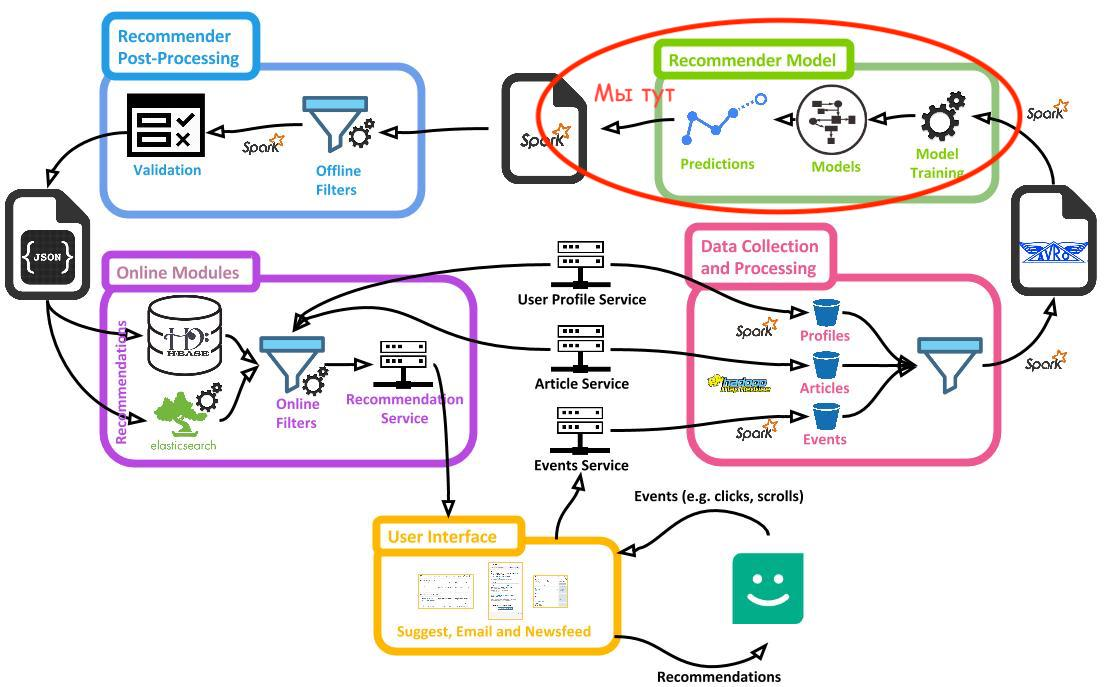
\includegraphics[scale=0.23]{images/mendeley.jpeg}
\end{center}

\end{frame}

\section{Графы и рекомендации}

\begin{frame}{Почему графы}

\begin{center}

\includegraphics[scale=0.4]{images/graphs.jpeg}
\end{center}

\end{frame}

{
\usebackgroundtemplate{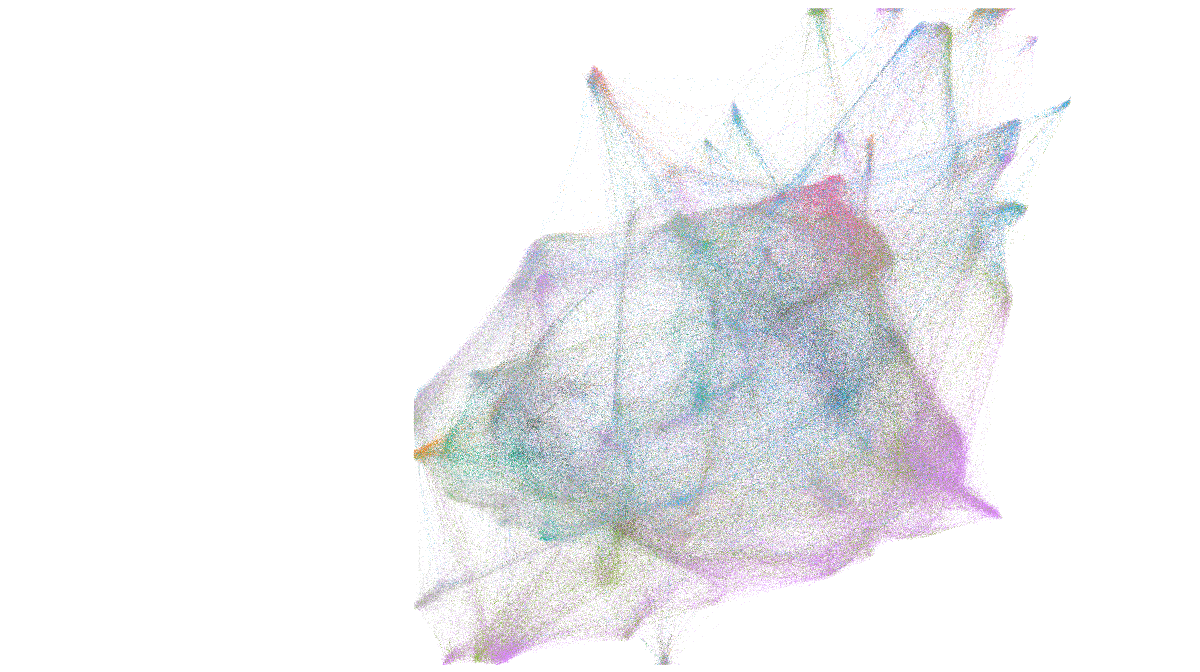
\includegraphics[width=\paperwidth]{images/ok-music-graph.png}}
\begin{frame}[plain]{Граф исполнителей в Одноклассниках}

20000 вершин \\
750000 ребер

\vspace{1em}

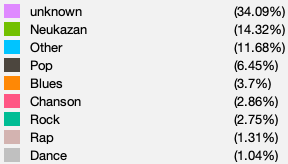
\includegraphics[scale=0.4]{images/ok-music-graph-legend.png}

\end{frame}
}

\section{Классика}

\begin{frame}{Personalized Page Rank (PPR) \cite{PPR}}

\begin{columns}
\begin{column}{0.4\textwidth}
\begin{center}
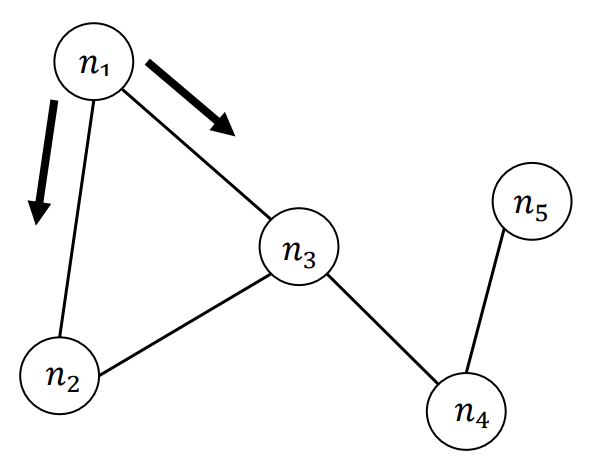
\includegraphics[scale=0.4]{images/example-graph.png}
\end{center}
\end{column}

\begin{column}{0.5\textwidth}
\begin{footnotesize}
Начальное состояние
\[
\vec{s}_0 = \begin{pmatrix}
	1 & 0 & 0 & 0 & 0
\end{pmatrix}
\]

Вероятность перехода
\[
\vec{p}_{n+1} = c \vec{s}_n \cdot P + (1 - c) \vec{s}_0 
\]
\[
P = \begin{pmatrix}
	0 & 1/2 & 1/2 & 0 & 0 \\
	1/2 & 0 & 1/2 & 0 & 0 \\
	1/3 & 1/3 & 0 & 1/3 & 0 \\
	0 & 0 & 1/2 & 0 & 1/2 \\
	0 & 0 & 0 & 1 & 0
\end{pmatrix}
\]
$(1-c)$ -- вероятность рестарта
\end{footnotesize}
\end{column}

\end{columns}

\vfill

\begin{tcolorbox}[colback=blue!5,colframe=blue!70,title=]
Где мы окажемся через бесконечное число шагов?
\end{tcolorbox}

\end{frame}

\begin{frame}{Вычисление рекомендаций}

\begin{columns}

\begin{column}{0.5\textwidth}
\begin{itemize}[<+->]
\item Точное решение
\[
\vec{r} = c \vec{r} P + (1 - c) \vec{s} \quad \Rightarrow \quad
\]
\[
\vec{r} = (1 - c) \vec{s} \left(I - c P \right)^{-1}
\]
\item Сэмплирование Монте-Карло
\item Оптимизированное прямое решение
\item Оптимизированный power iteration
\end{itemize}
\end{column}

\begin{column}{0.4\textwidth}
\begin{center}
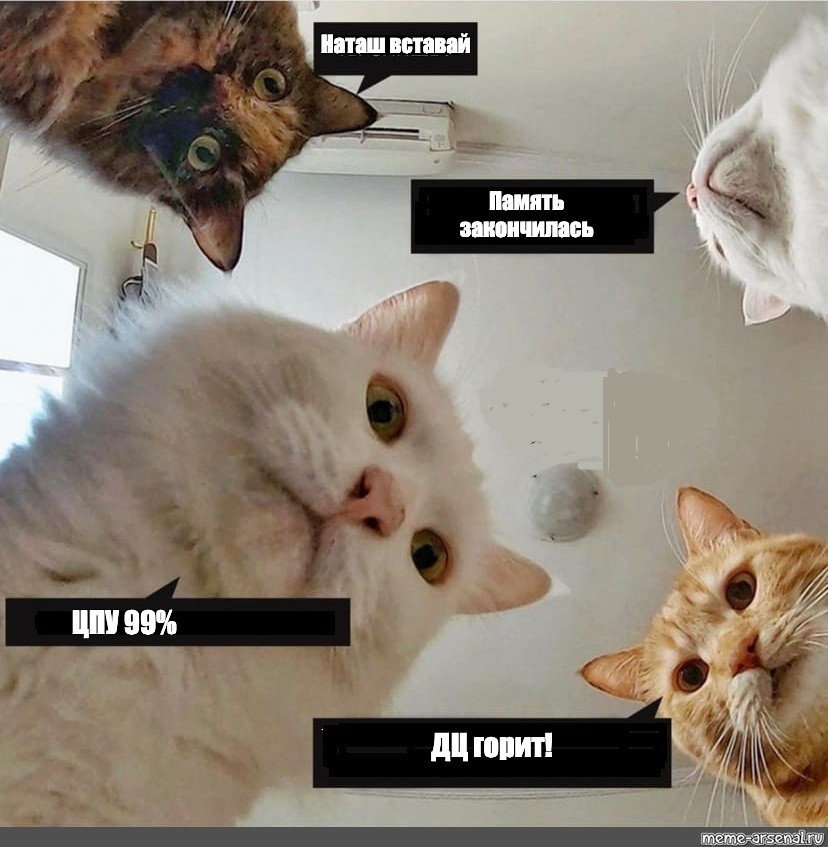
\includegraphics[scale=0.2]{images/natash.jpeg}
\end{center}
\end{column}

\end{columns}

\end{frame}

\section{Молниеносное введение в GNN}

\begin{frame}{Разные виды данных в нейросетях \cite{GNN}}

\begin{center}
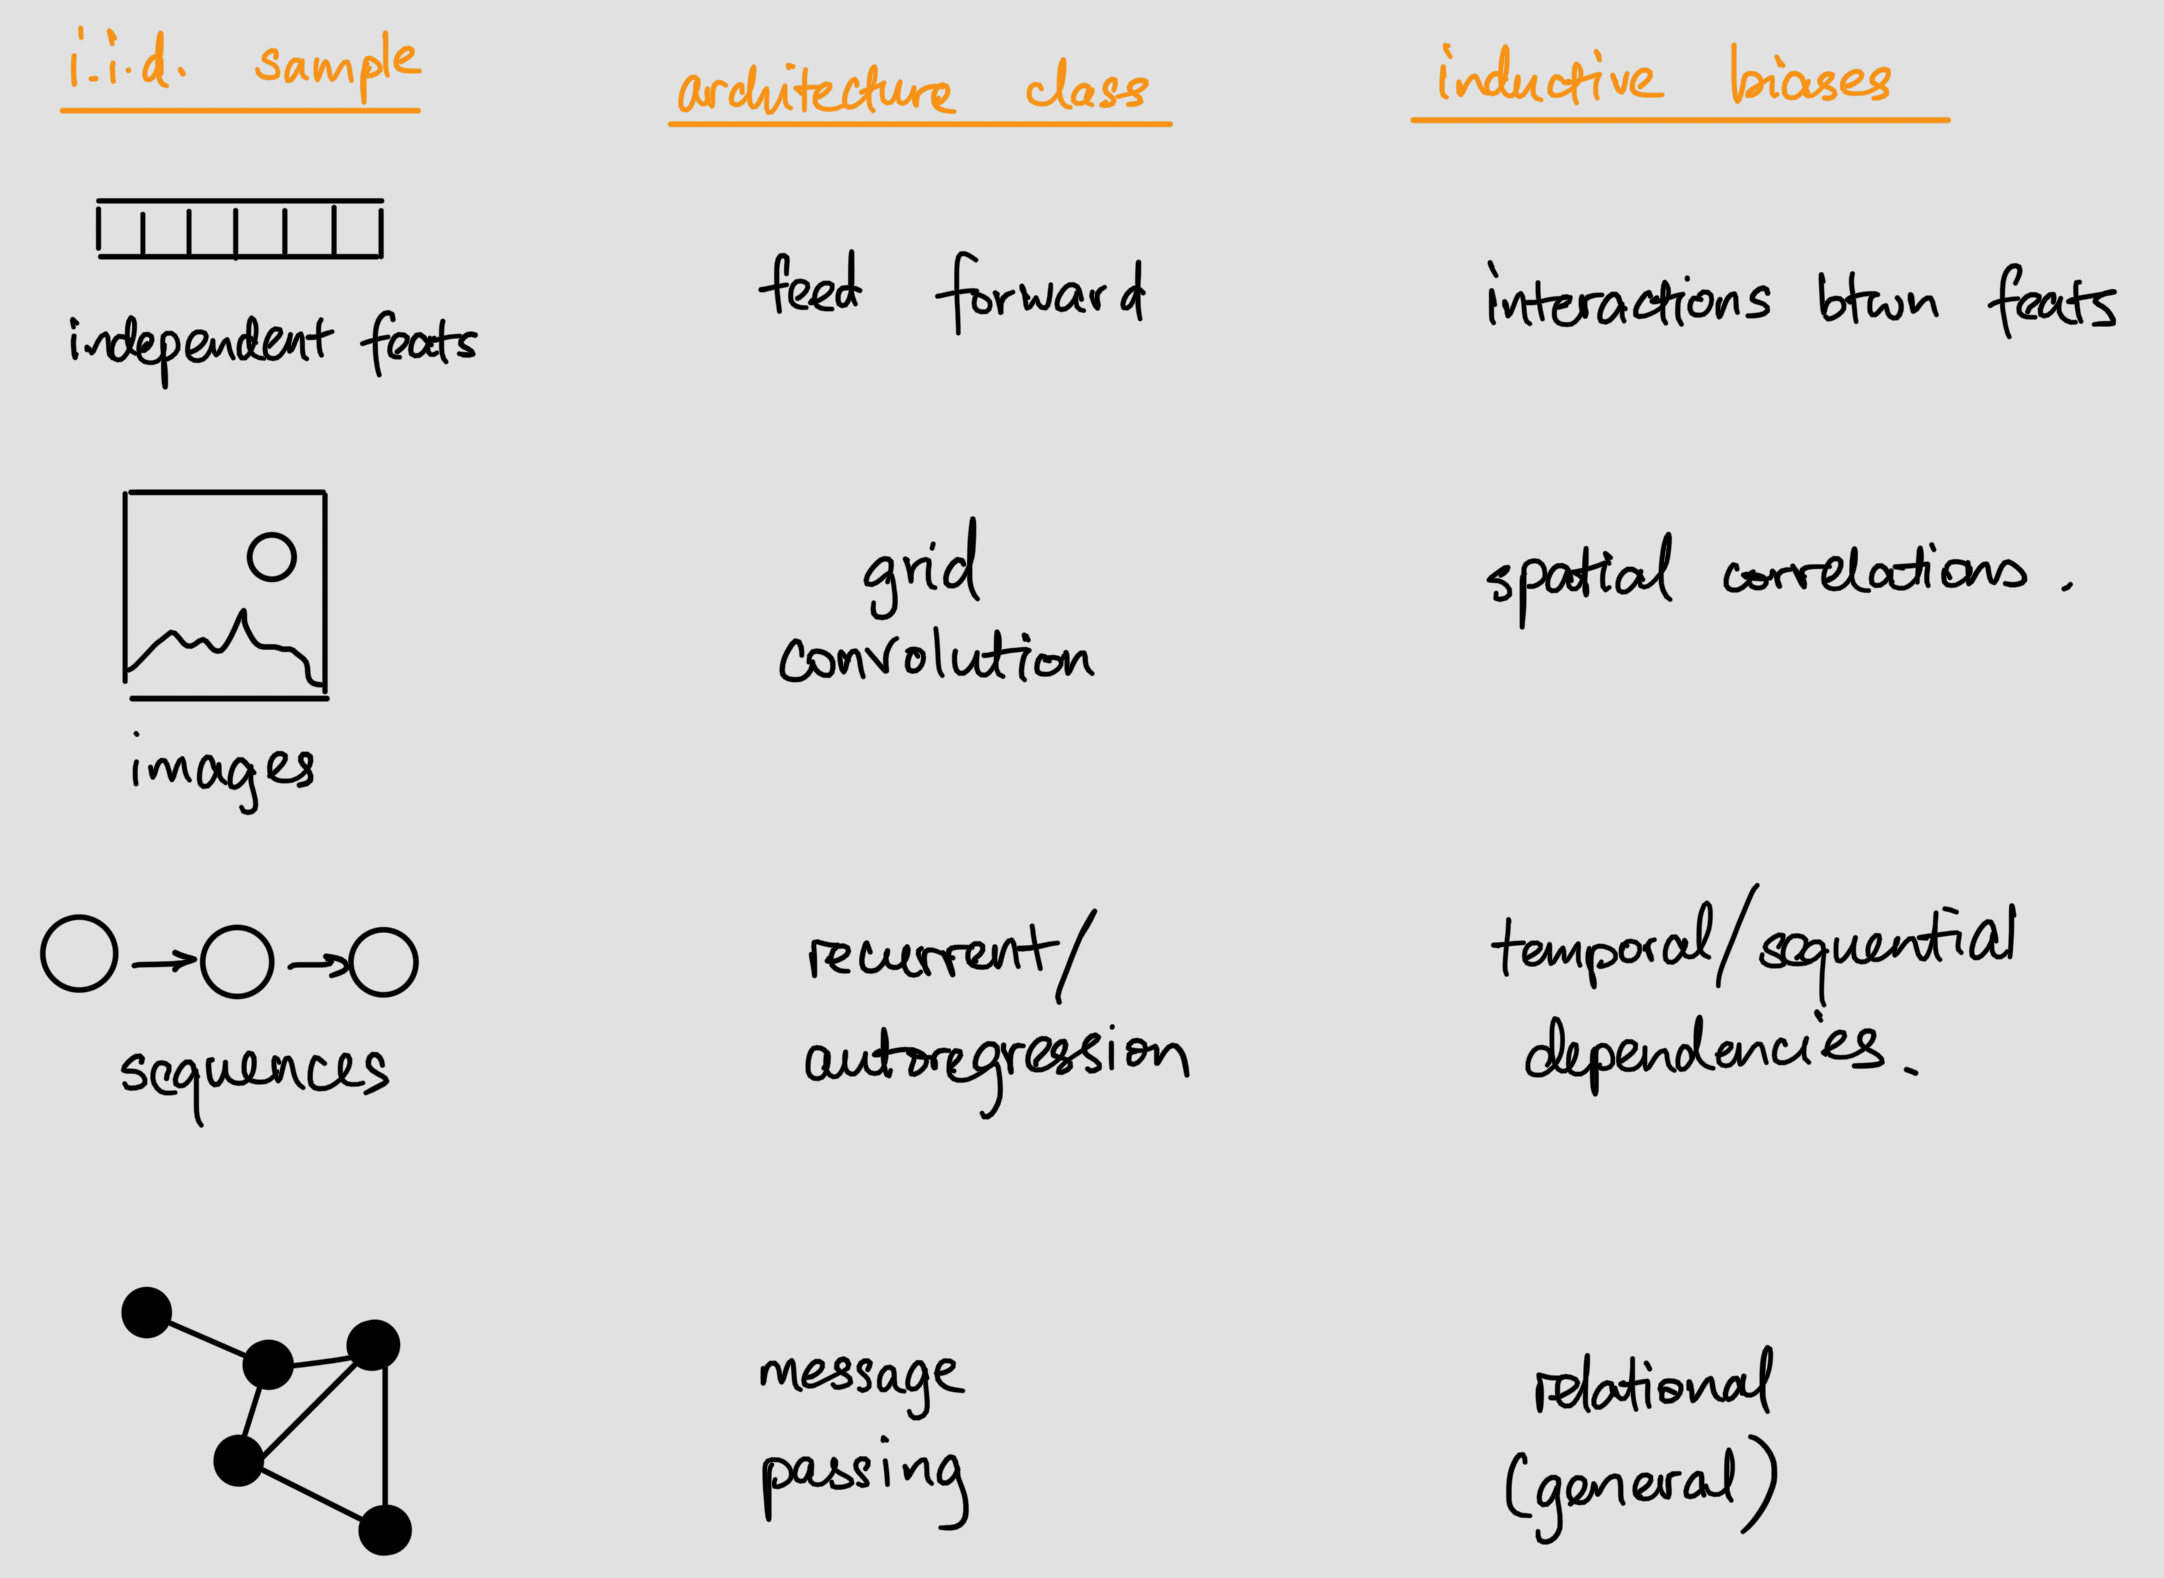
\includegraphics[scale=0.12]{images/inductive-biases.png}
\end{center}

\end{frame}

\begin{frame}{Признаки узлов}

\begin{center}
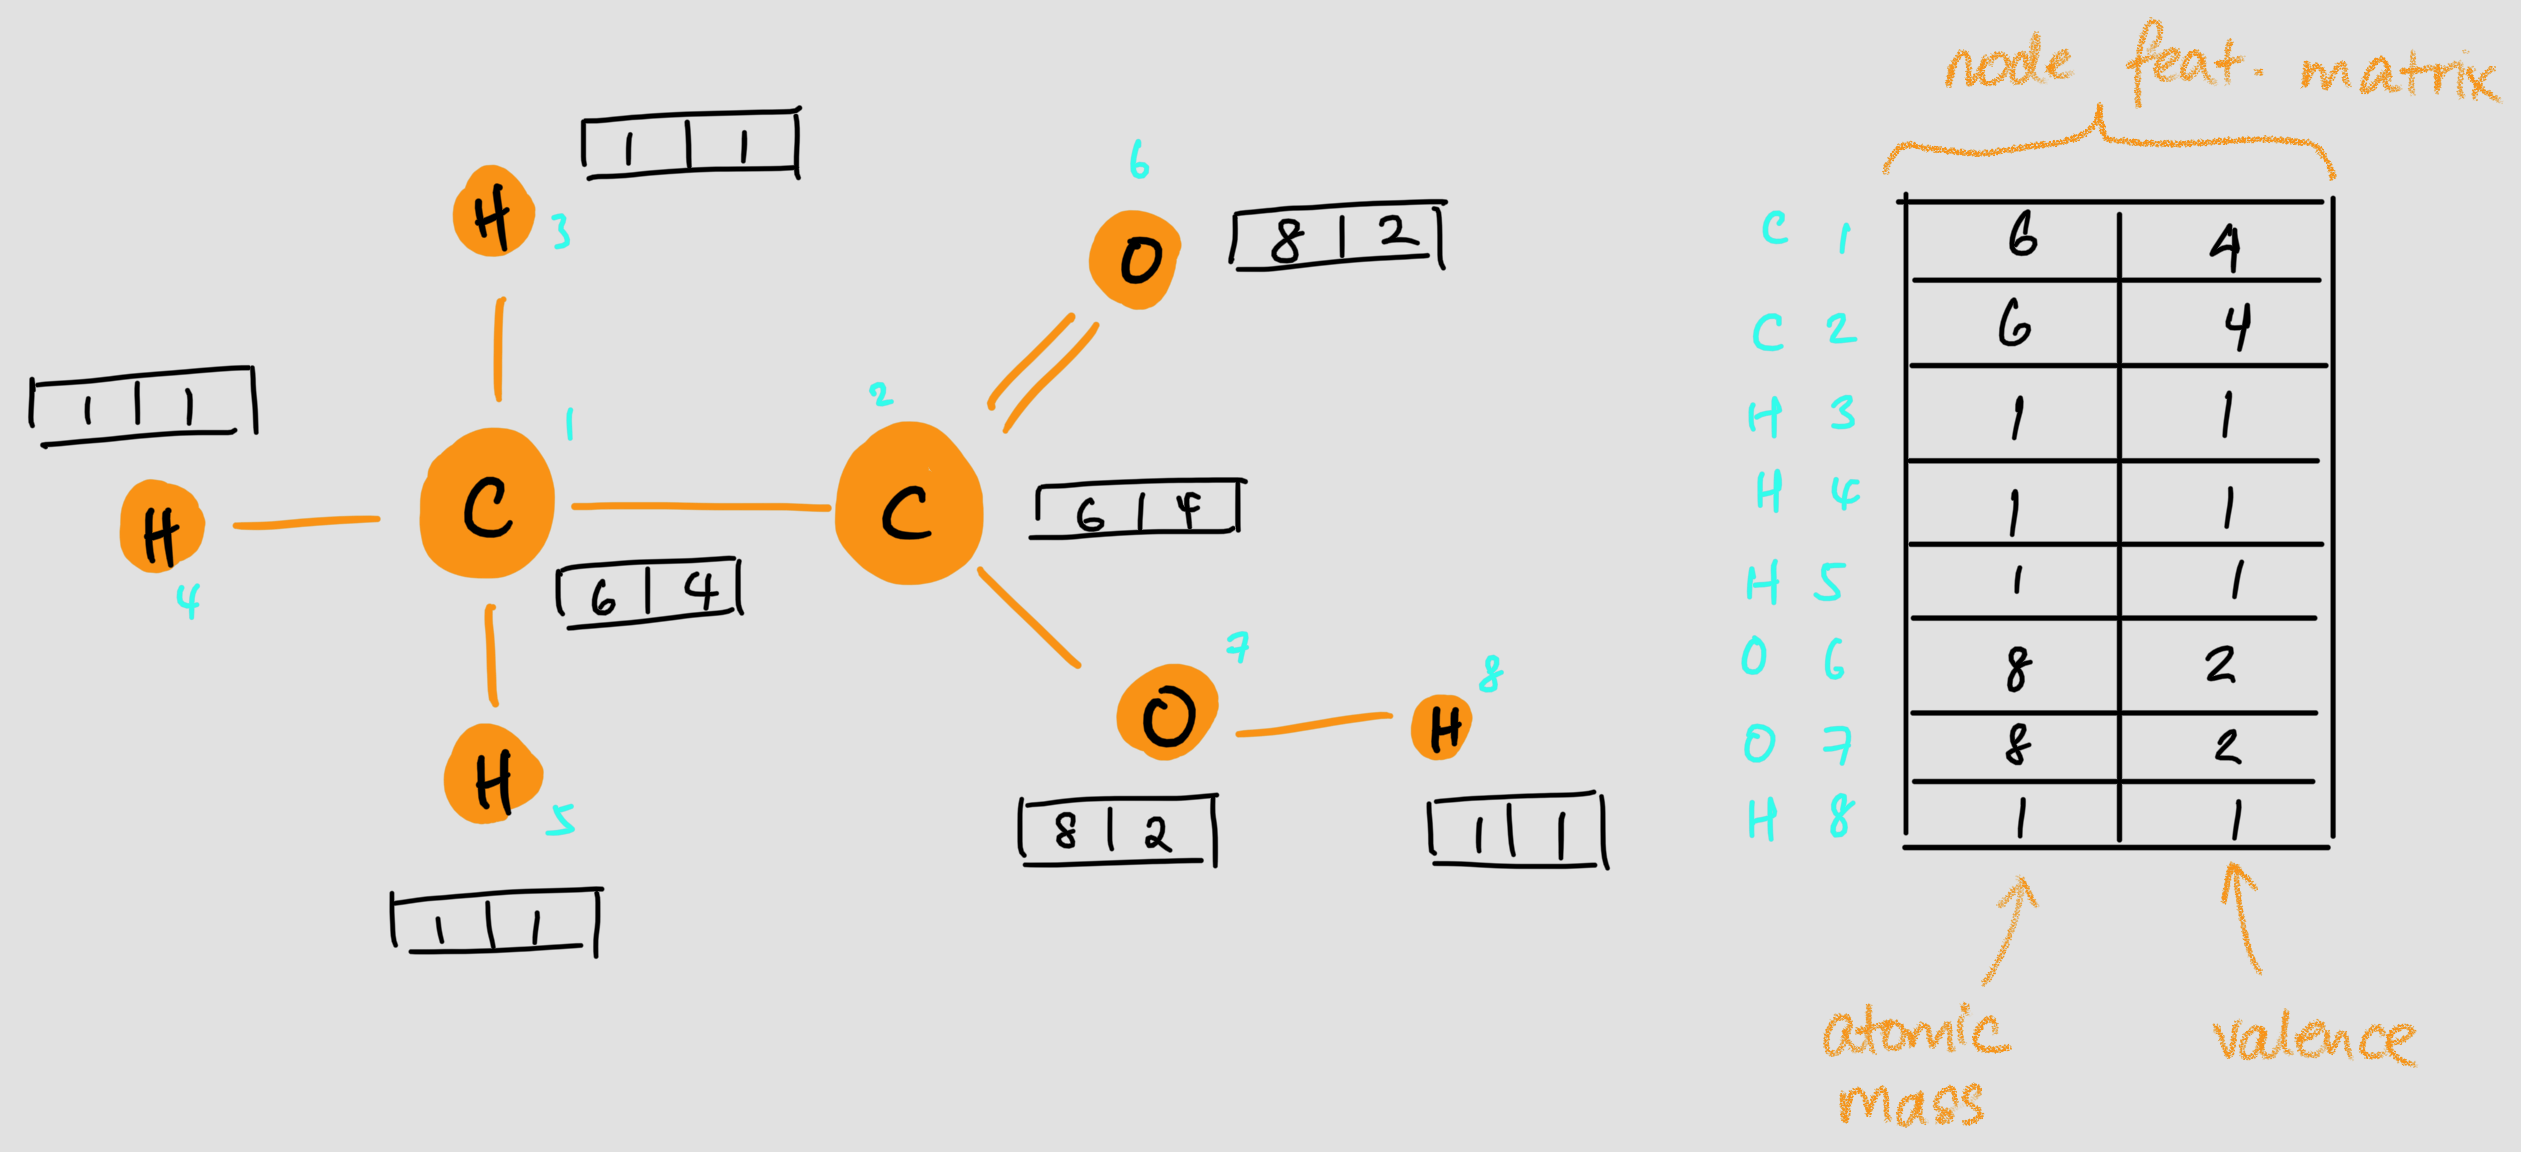
\includegraphics[scale=0.15]{images/ethanoic-acid-features.png}
\end{center}

\end{frame}

\begin{frame}{Структура графа}

\begin{center}
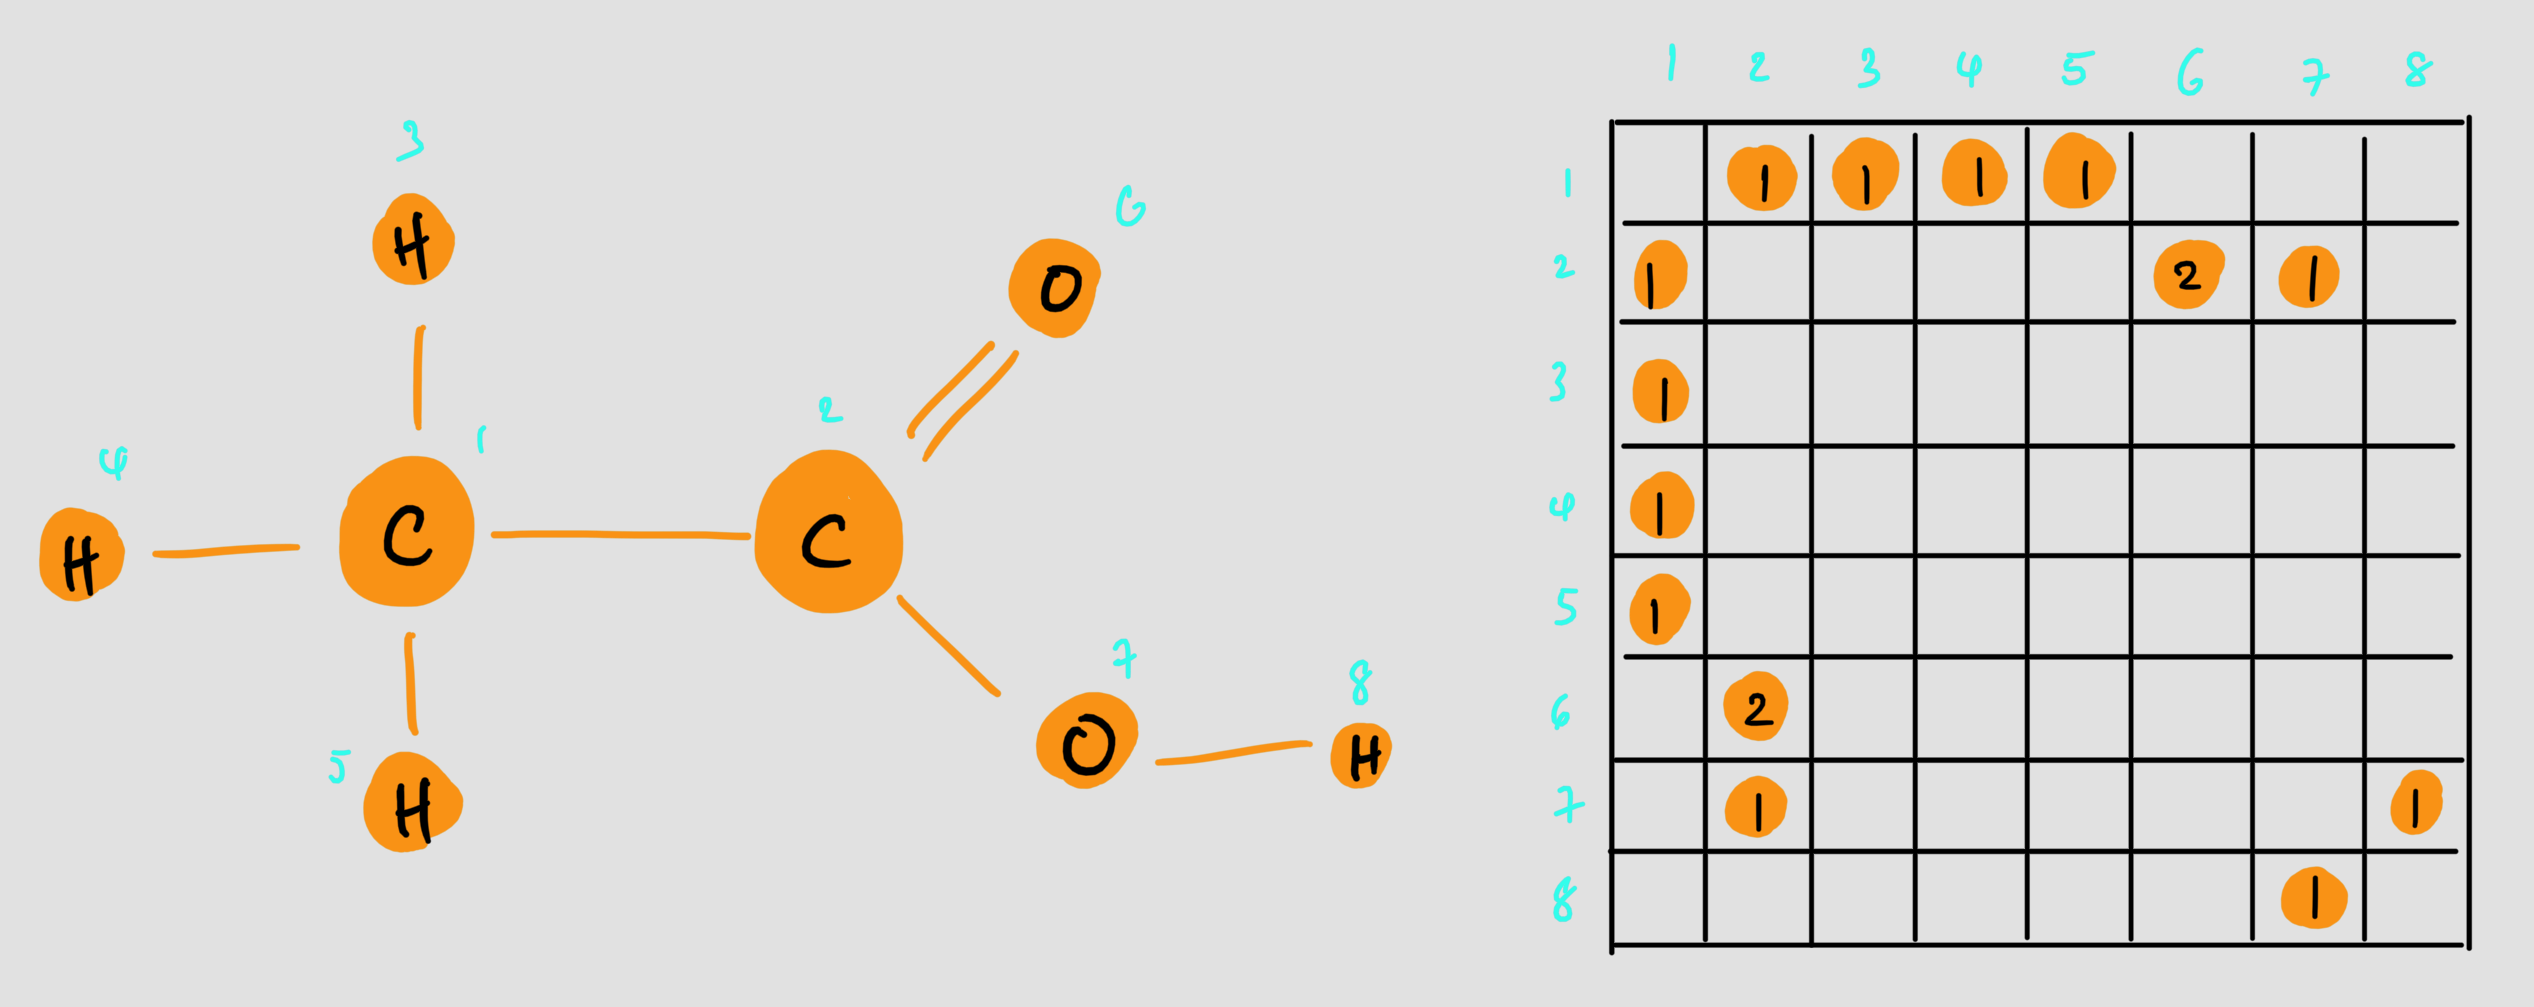
\includegraphics[scale=0.15]{images/ethanoic-acid-weighted-adjacency.png}
\end{center}

\end{frame}

\begin{frame}{Интуиция message passing}

\begin{center}
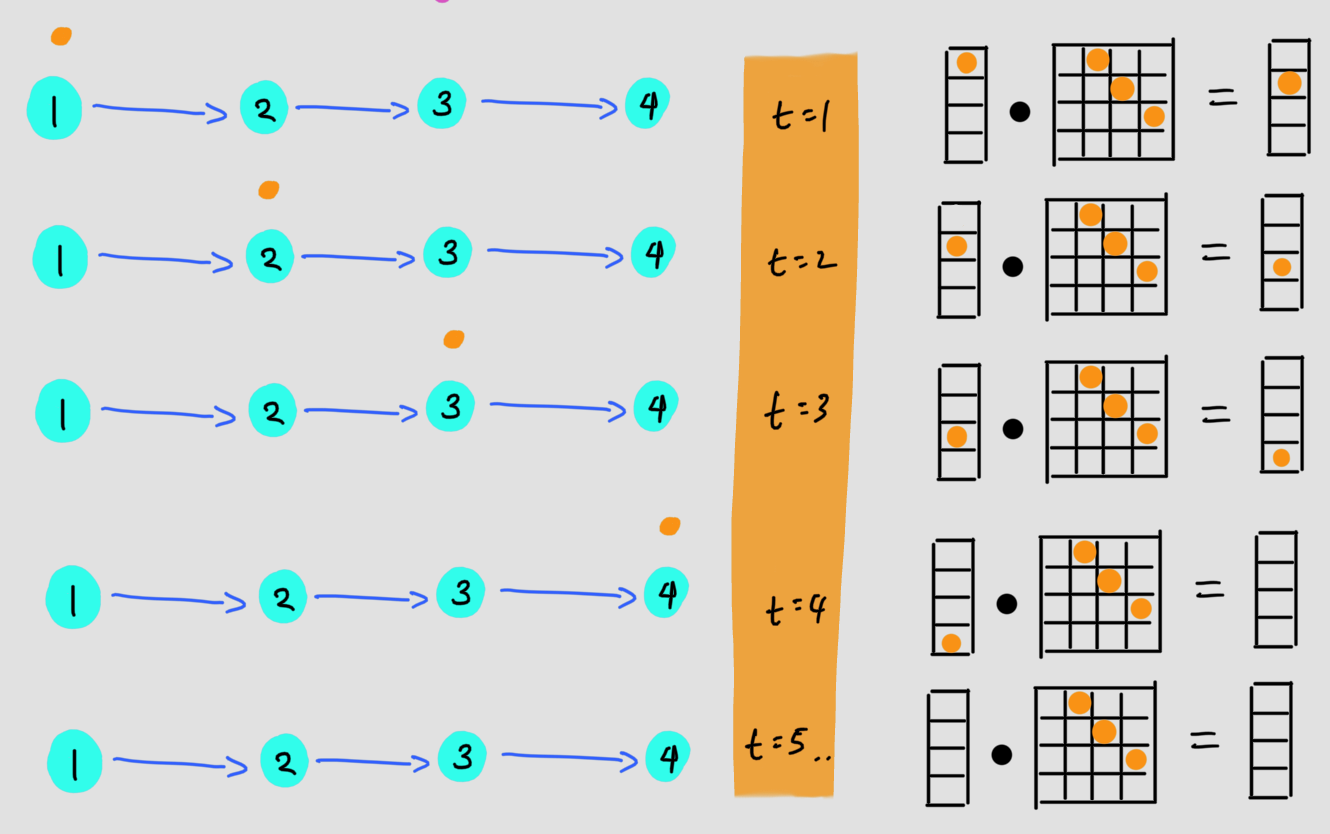
\includegraphics[scale=0.24]{images/message-passing-chain.png}
\end{center}

\end{frame}

\begin{frame}{Message passing}

\begin{center}
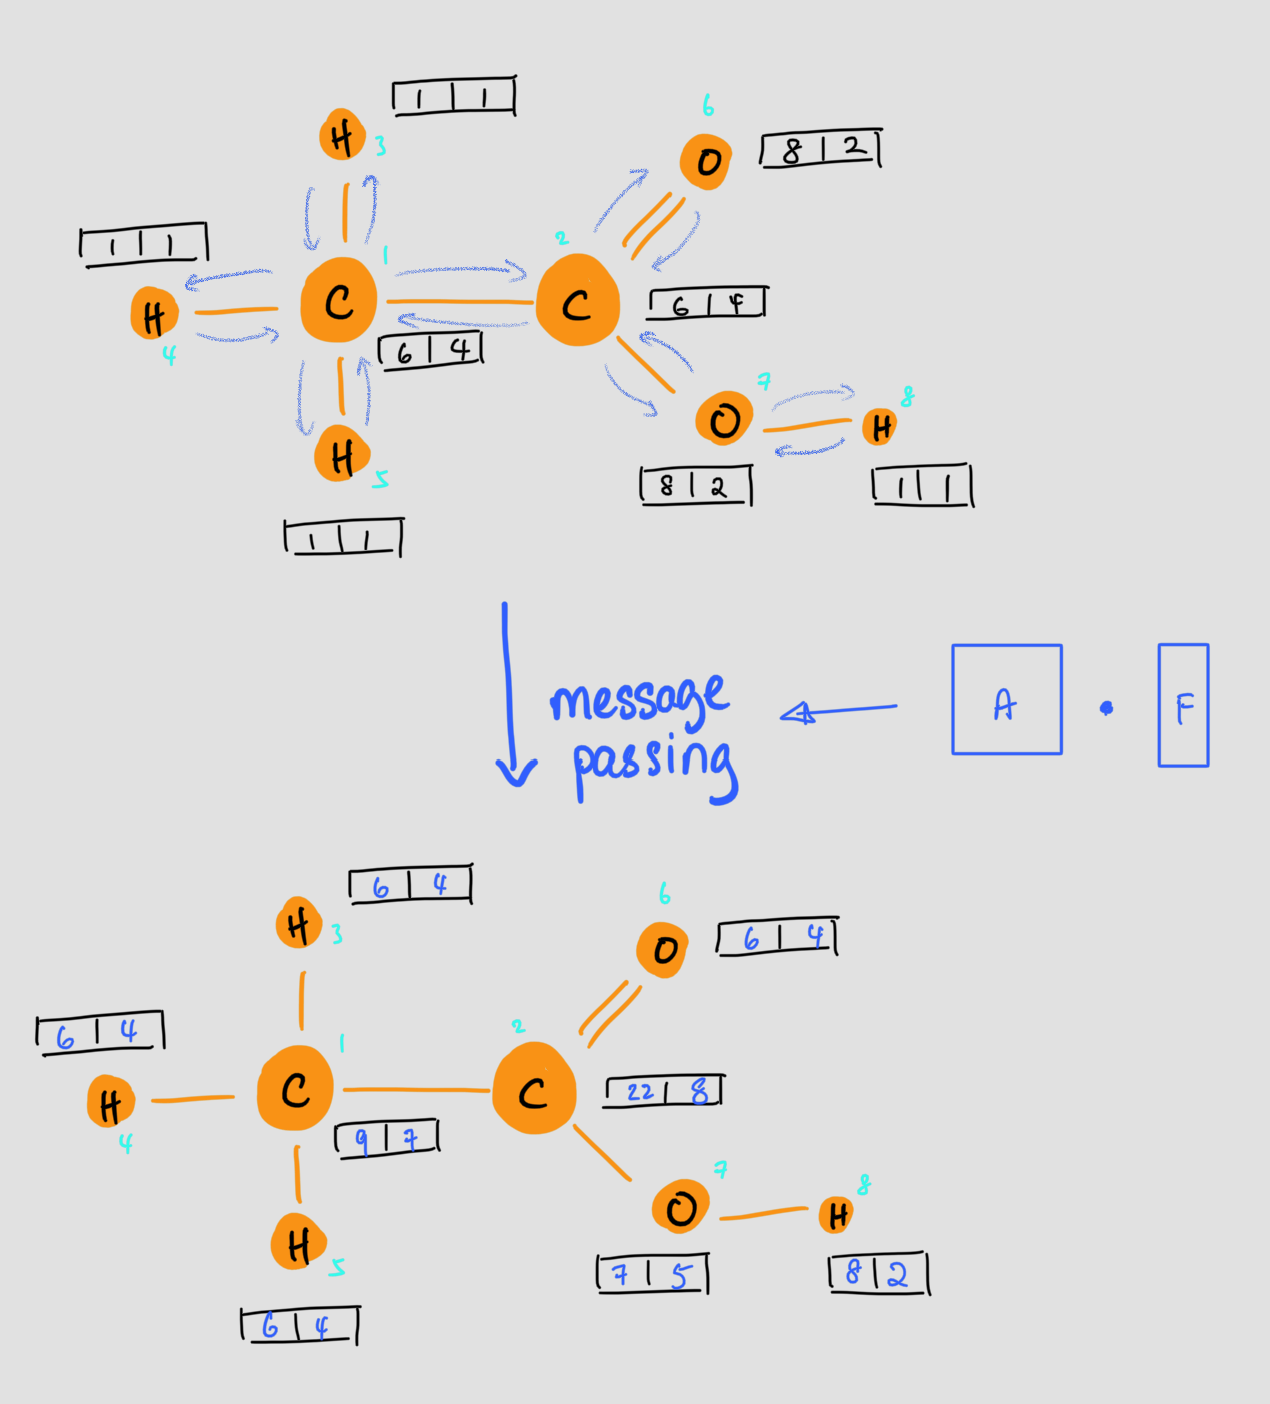
\includegraphics[scale=0.13]{images/message-passing-ethanoic-acid.png}
\end{center}

\end{frame}

\begin{frame}{А где же нейросети?}

\begin{center}
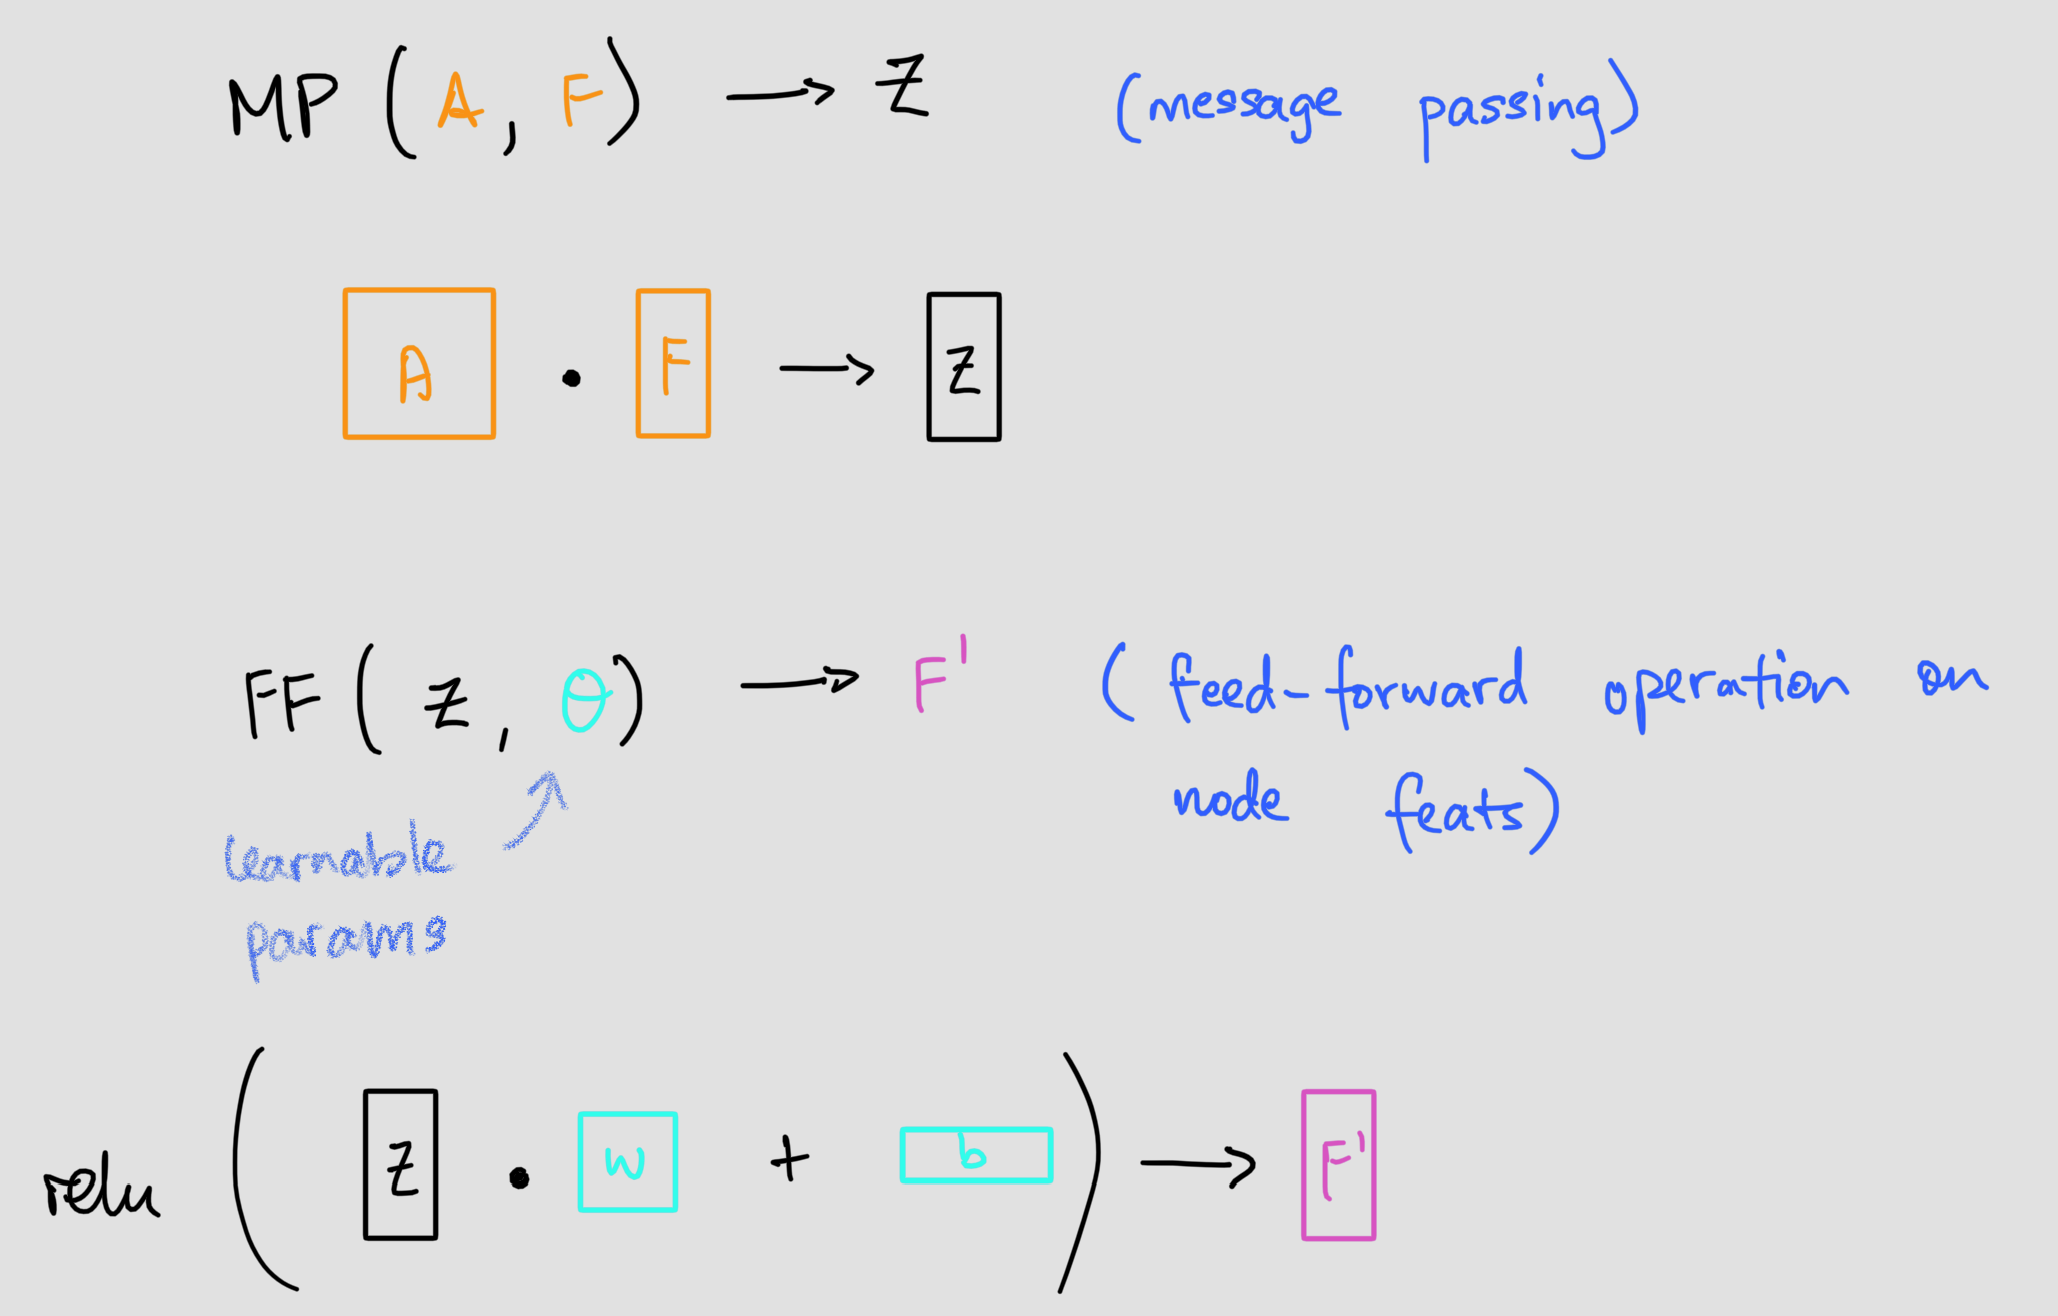
\includegraphics[scale=0.15]{images/message-passing-layer.png}
\end{center}

\end{frame}

\begin{frame}{Общий фреймворк GNN \cite{GNNSURVEY}}

{\bf A.} Message passing в узле $n_v^{(l)}$ на $l$ слое:
\begin{enumerate}
\item Агрегация представлений соседей $h_u^{(l)}$ (Aggregation)
\[
n_v^{(l)} = Aggregator_l(\{h_u^{(l)}, u \in N(v)\}), 
\]
\item Апдейт представления
\[
h_v^{(l+1)} = Updater_l(n_v^{(l)}, h_v^{(l)})
\]
\end{enumerate}

\pause

{\bf B.} Использование представлений узлов для решения задачи
\begin{itemize}
\item Классификация узлов $f(h_v)$
\item Предсказание / классификация связей $g(h_v \cdot h_u)$
\item Классификация графов $h(Pooling(h_v))$
\end{itemize}

\end{frame}

\begin{frame}{Примеры GNN}

GraphSage

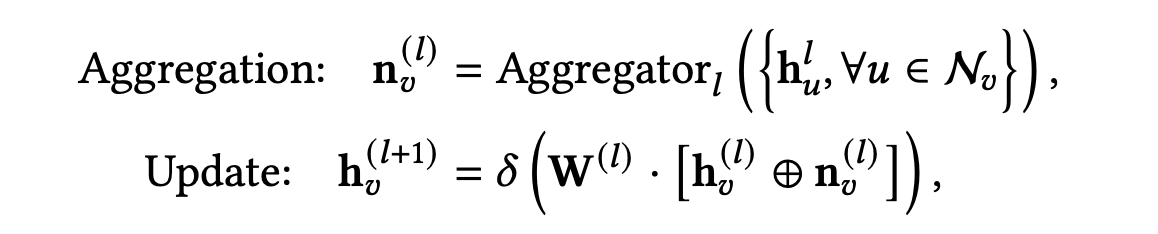
\includegraphics[scale=0.4]{images/graphsage.png}

GAT

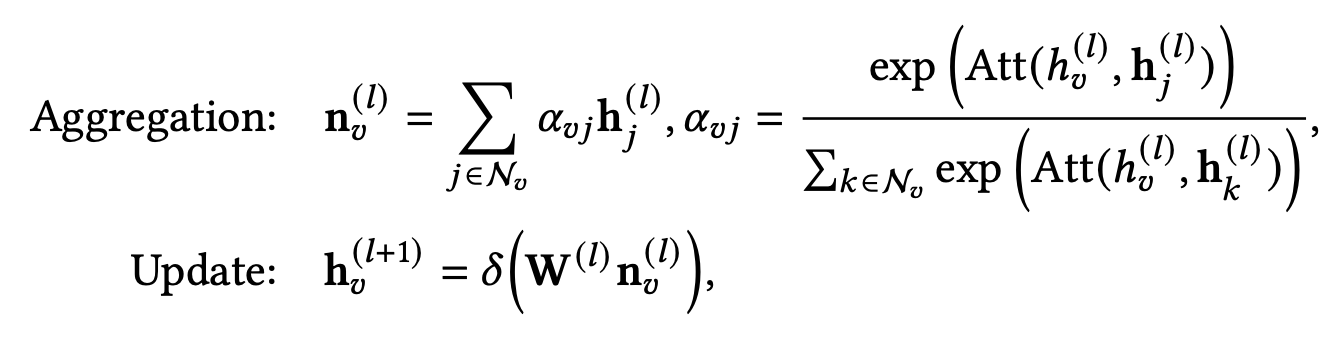
\includegraphics[scale=0.4]{images/gat.png}

\end{frame}

\section{GNN в рекомендациях}

\begin{frame}{GNN в рекомендациях \cite{GNNSURVEY}}

\begin{center}
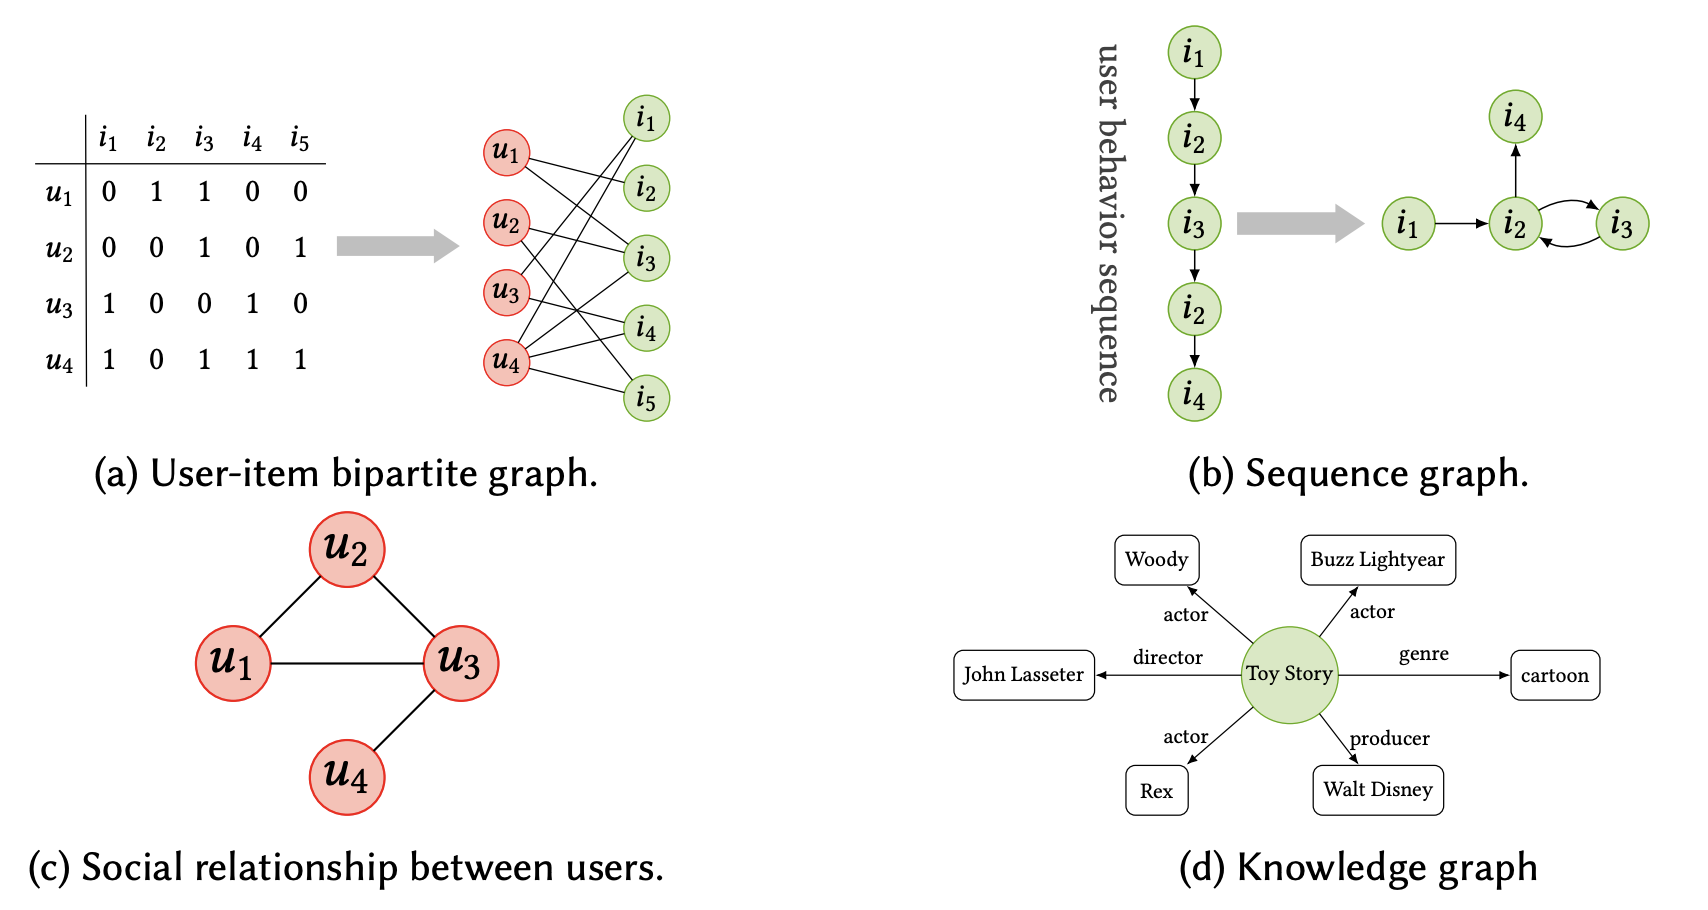
\includegraphics[scale=0.3]{images/gnn-rec-problems.png}
\end{center}

\end{frame}

\begin{frame}{GNN для коллаборативной фильтрации}

\begin{center}
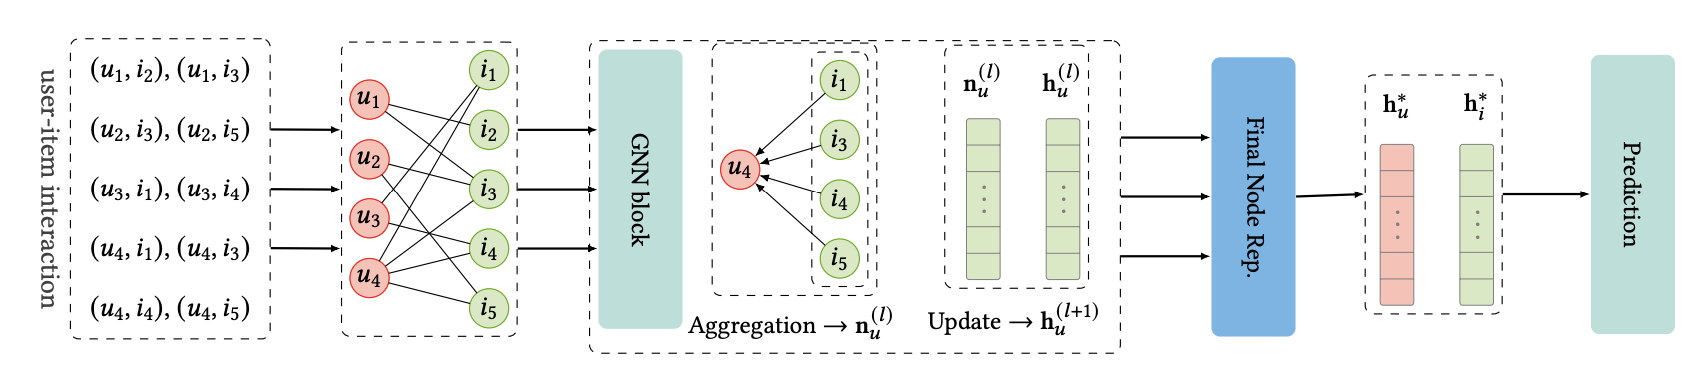
\includegraphics[scale=0.3]{images/gnn-cf.png}
\end{center}

Вопросы
\begin{itemize}
\item Как построить граф?
\item Как сформировать финальное представление пользователей и айтемов?
\end{itemize}

\end{frame}

\begin{frame}{GNN на последовательностях айтемов}

\begin{columns}
\begin{column}{0.5\textwidth}
\begin{center}
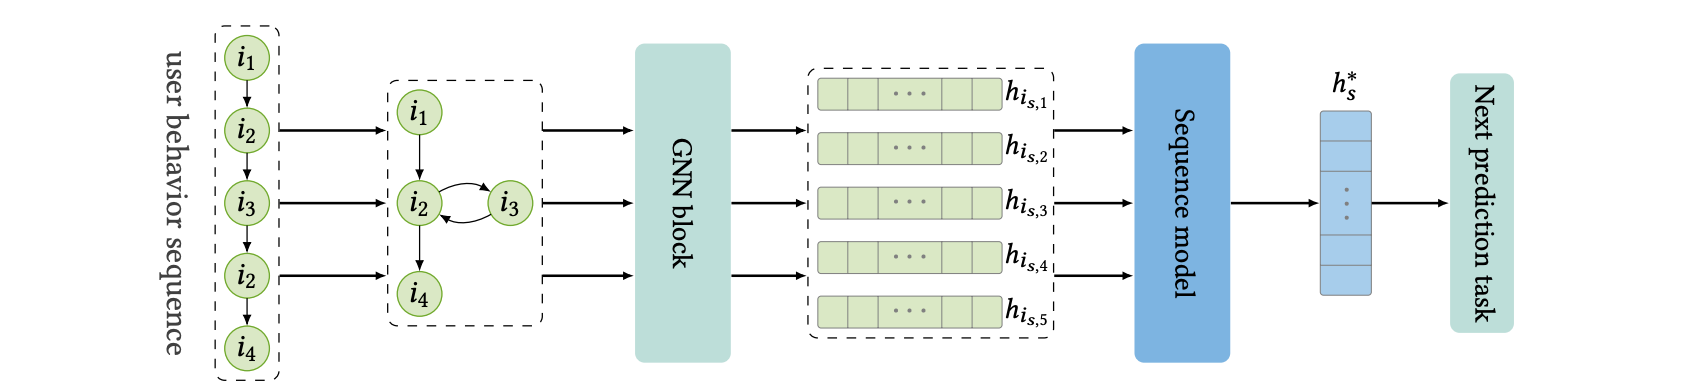
\includegraphics[scale=0.25]{images/gnn-seq.png}
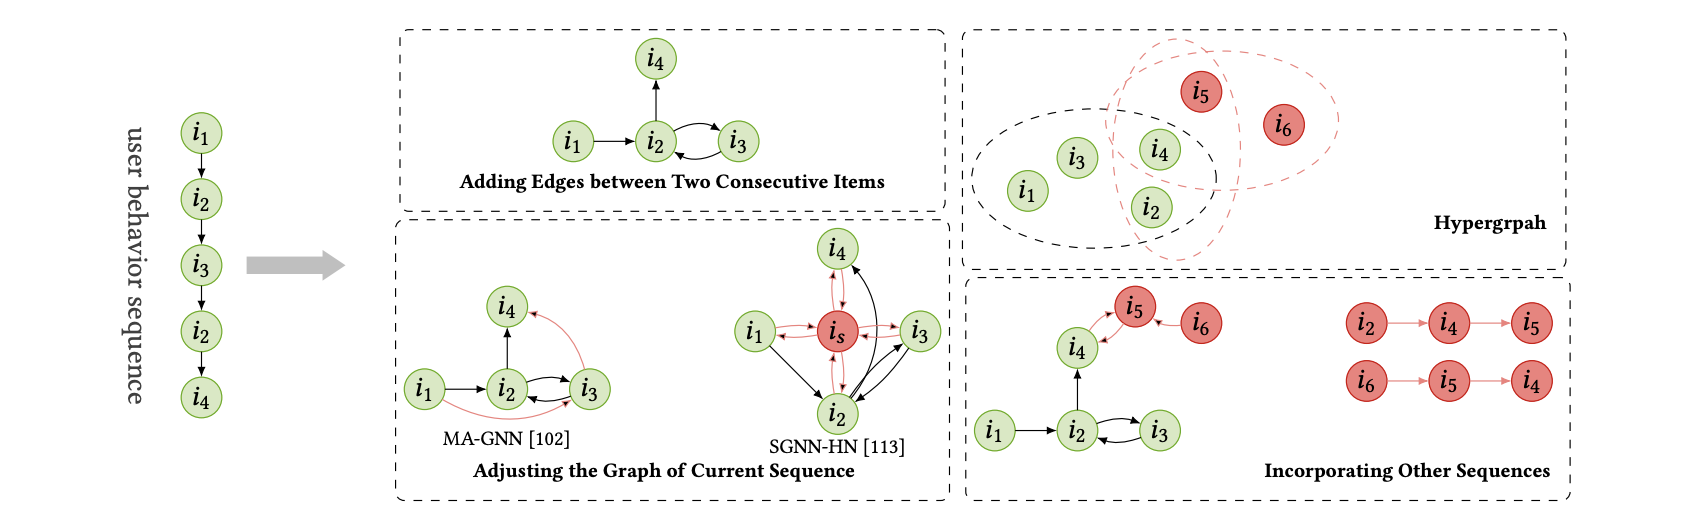
\includegraphics[scale=0.25]{images/gnn-seq-graph.png}
\end{center}
\end{column}

\begin{column}{0.4\textwidth}
Вопросы
\begin{itemize}
\item Как построить граф?
\item Как сагрегировать информацию всей последовательности?
\end{itemize}
\end{column}

\end{columns}

\end{frame}

\begin{frame}{GNN в задачах с соцсетью}

\begin{center}
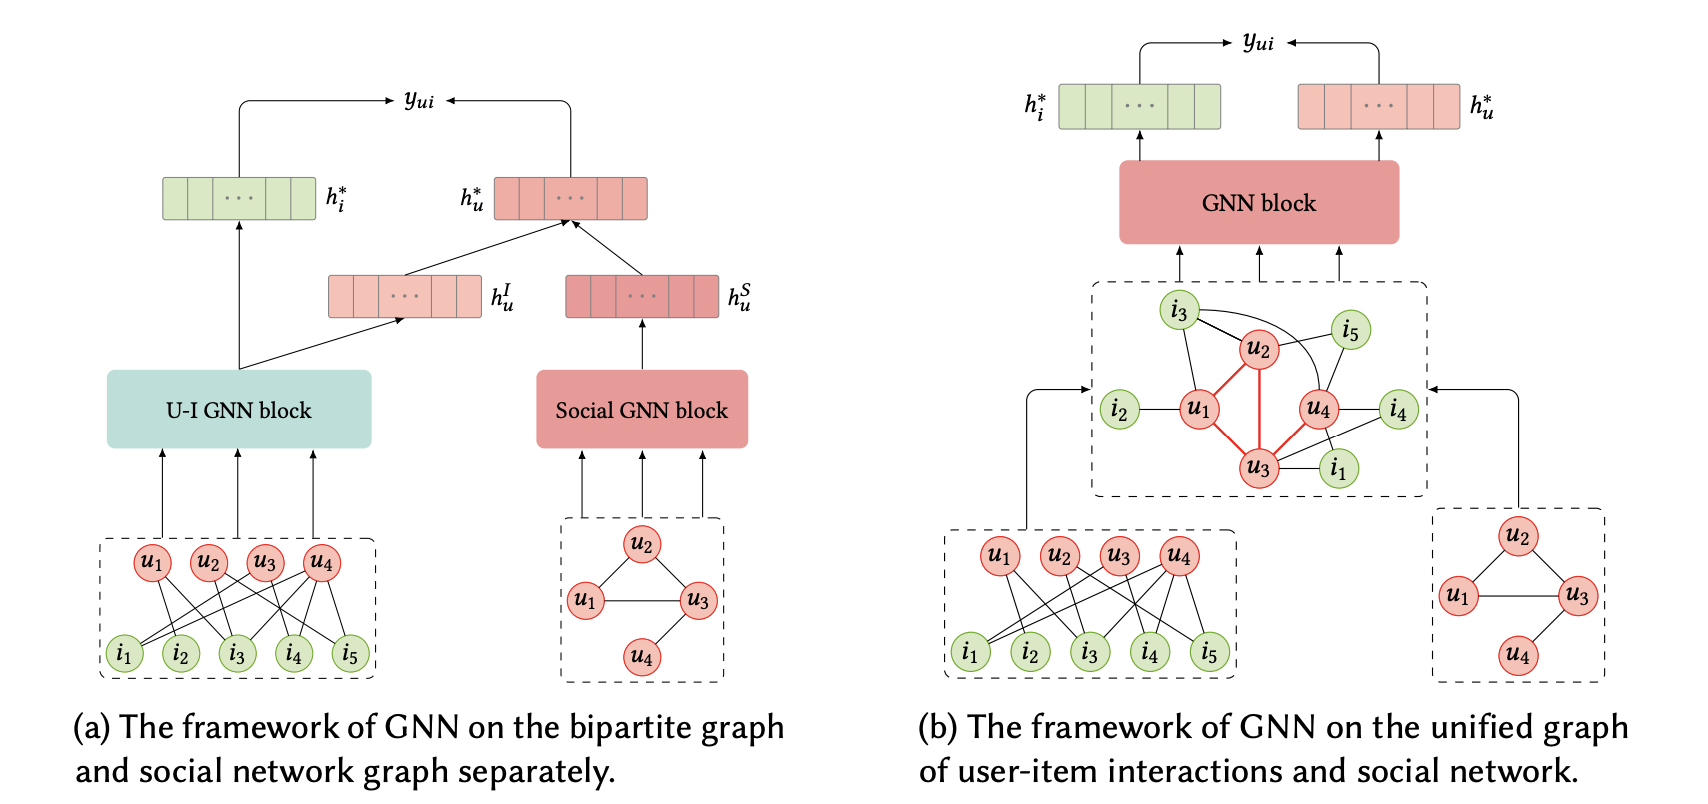
\includegraphics[scale=0.3]{images/gnn-social.png}
\end{center}

Вопросы
\begin{itemize}
\item Комбинировать ли граф CF с графом друзей?
\item Разный ли вес у друзей?
\end{itemize}

\end{frame}

\begin{frame}{GNN в задачах с графом знаний}

PinSage: A new graph convolutional neural network for web-scale recommender systems \cite{PINSAGE}

\begin{center}
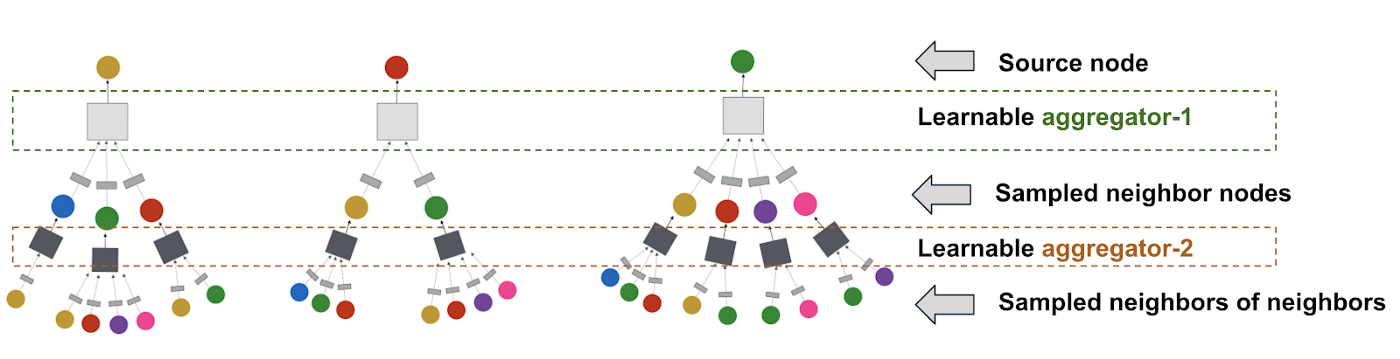
\includegraphics[scale=0.3]{images/pinnersage.png}
\end{center}

\end{frame}

\begin{frame}{А вообще работает?}
LightGCL: Simple Yet Effective Graph Contrastive Learning for Recommendation
 \cite{LIGHTGCL}
 
\begin{center}
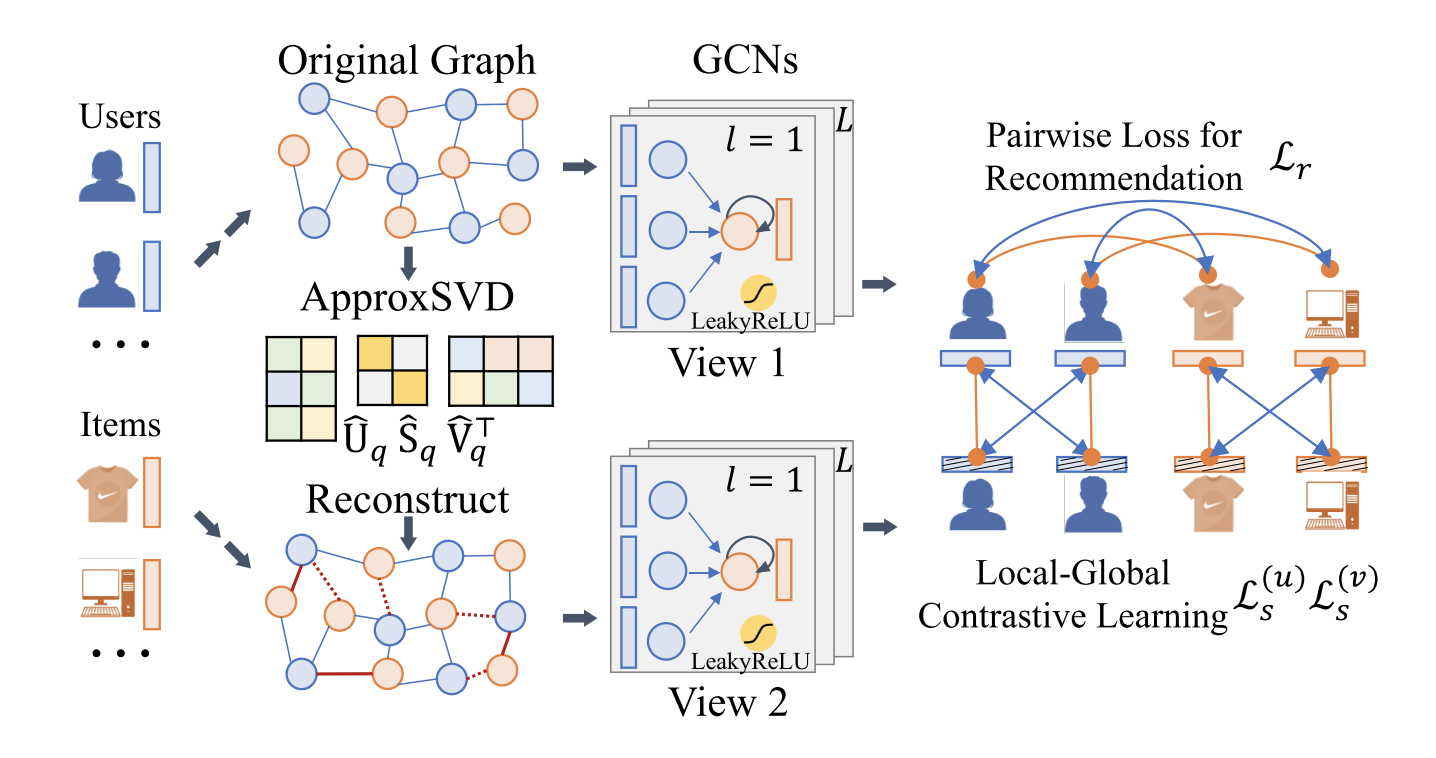
\includegraphics[scale=0.3]{images/lightgcl.png}
\end{center}

\end{frame}

\begin{frame}
 
\begin{center}
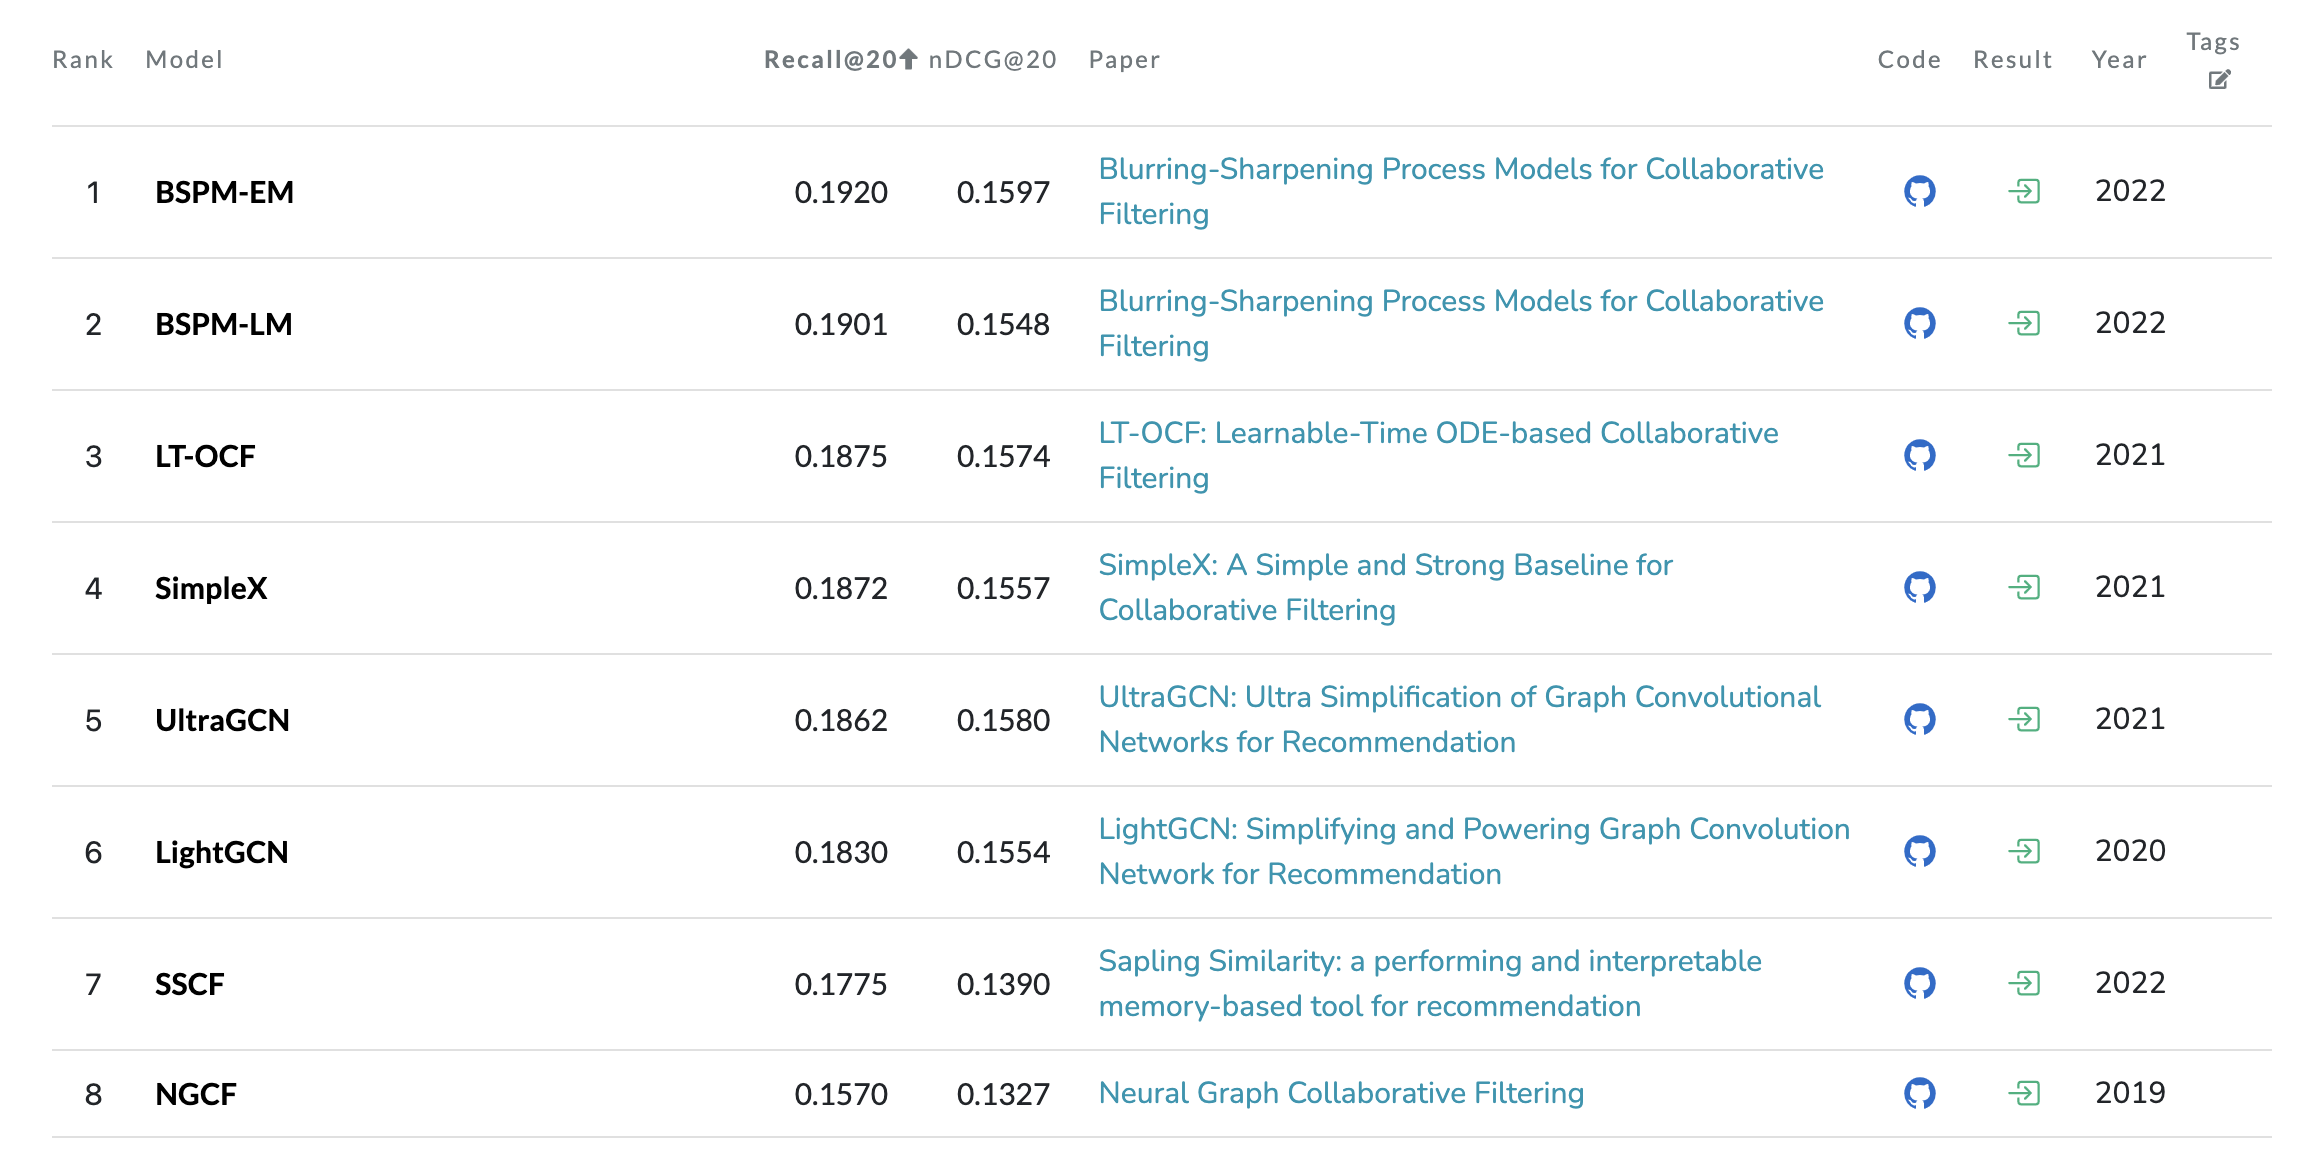
\includegraphics[scale=0.3]{images/pwc.png}
\end{center}

\url{https://paperswithcode.com/sota/recommendation-systems-on-gowalla}

\end{frame}

\begin{frame}
 
\begin{center}
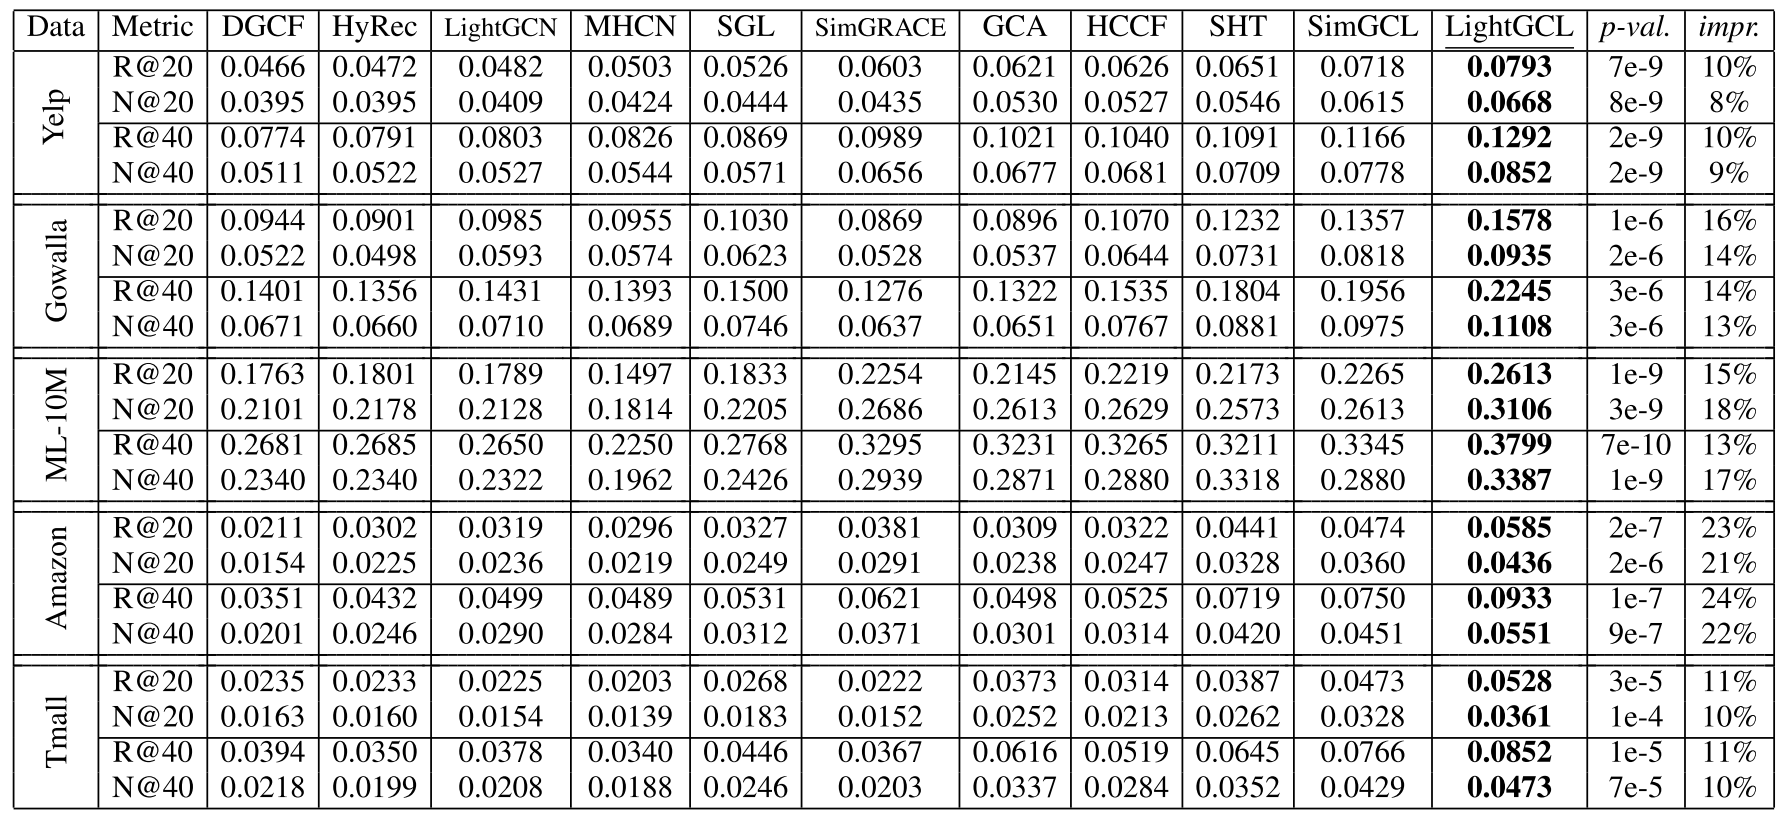
\includegraphics[scale=0.3]{images/lightgcl-exp.png}
\end{center}

\end{frame}

\section{Итоги}

\begin{frame}{Итоги}

\begin{tcolorbox}[colback=info!5,colframe=info!80,title=]
Архитектура GNN хорошо ложится на формулировку рекомендательной задачи.
\end{tcolorbox}

\begin{tcolorbox}[colback=warn!5,colframe=warn!80,title=]
Хотя это популярное направление в исследовательских статьях, польза от применения на продакшене пока что под вопросом.
\end{tcolorbox}

\end{frame}

\begin{frame}{До следующего раза}

\begin{columns}
\begin{column}{0.45\textwidth}
   \begin{center}
                
\includegraphics[scale=0.25]{images/bye.png}
   \end{center}
\end{column}
\begin{column}{0.45\textwidth}
   \begin{center}
                \url{https://t.me/mlvok}

                
\includegraphics[scale=0.5]{images/tgqr.png}
   \end{center}
\end{column}
\end{columns}

\end{frame}

\begin{frame}[allowframebreaks]{Литература}

\bibliographystyle{amsalpha}
\bibliography{references.bib}

\end{frame}

\end{document}
